\chapter{Magnolia IDE} \label{cha:ide}

This section will discuss the new Magnolia \gls*{ide}, the different users of the
\gls*{ide}, and their possible experiences which was under consideration when
developing the application.

\section{User Perspectives}

This application has to consider different users. In \gls*{ide}'s like
\gls*{eclipse} or \gls*{intellij}, there is the primary user base, the developers
who are using the \gls*{ide} to develop, and then there are the secondary user
base, the developers whom develop \textit{plugins} for the \gls*{ide}. Being the
primary user base, most of the new features implemented by either \gls*{ide} are
related to the development experience. There are still changes to that the
\textit{plugin} developers are interested in, namely \gls*{api} changes.
\gls*{intellij} for example, lists their \textit{incompatible \gls*{api} changes}~\cite{intellijBrokenApi}.
Breaking changes between \gls*{ide} versions is something normal users of the
\gls*{ide} do not worry about. As usually when a new version is released, it
means more features for the developer to utilize. While \textit{plugin}
developers have to ensure their \textit{plugins} still work. One of the reasons
behind \gls*{ide} version changes can break a \textit{plugin}, is due to how
they interact with their \gls*{ide}. In \gls*{intellij} a \textit{plugin} is
created by implementing a Java interface for the functionality one wants.

If one wanted \gls*{intellij} to recognize that a file with the extension "rs",
is a Rust source file, and give it a certain icon, one would have to implement
the \textbf{Language} interface and override the \textbf{getIcon} method to
return the wanted icon.

So a change in the \gls*{ide} architecture could break a \textit{plugin} for the
newer version of the \gls*{ide}, as with Bagge's Magnolia \gls*{ide}~\cite{baggeIde}.
While in this zero core \gls*{ide} module developers are quite important, as they
are the ones who add the functionality to the \gls*{ide}. Therefore, the core
\gls*{api} has to be more stable, and it is by virtue of not having much
functionality.

\section{Module Developer}

Being a zero core application; all functionality comes from modules, the module
developer experience is the most important. To achieve this, documentation is
important. If a module developer has a question about how the core might react,
it should be answered by the documentation. In \gls*{eclipse}, this is in the
form of \textit{Javadoc}s, which specify, with examples how the \gls*{eclipse}
runtime handles \textit{plugins}. \footnote{\url{https://help.eclipse.org/latest/rtopic/org.eclipse.platform.doc.isv/reference/api/org/eclipse/core/runtime/Plugin.html}}

The documentation for \textit{plugin} developers, in both \gls*{intellij} and
\gls*{eclipse} has to be large, due to of how \textit{plugins} interact with the
\gls*{ide}; it is a large \gls*{api}. In a zero core \gls*{ide} it is smaller,
simply due to the fact that the core \gls*{ide} offers fewer features, as features
necessarily come from a module.

\subsection{Language Agnostic Modules}

The largest limiting factor in module oriented applications, is the
\textit{language barrier} Most applications limit what language one can extend
an application with, like in \gls*{vscode}, where its JavaScript/HTML/CSS. Or
\gls*{intellij}, where one can use Java or Kotlin. But what does language agnostic
mean in the context of programming languages? It is, and always will be C. Rust,
the language chosen to implement this \gls*{ide}, also has bindings to C. This
means that Rust can invoke C libraries. This is important for language
agnosticism, as any language that has bindings to C, has then, through C,
bindings to Rust. This is called an \gls*{abi}, specifically the C-\gls*{abi}.

\begin{figure}
  \begin{center}
    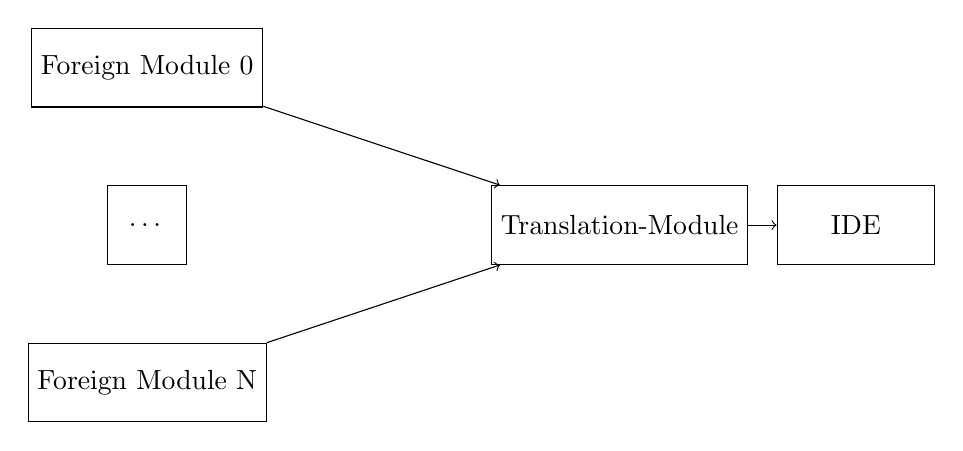
\begin{tikzpicture}
  % Nodes
  \node (p-0) [rectangle, draw, minimum height=1cm, minimum width=2cm] at (-6, 2) {Foreign Module 0};
  \node (dots) [rectangle, draw, minimum height=1cm, minimum width=1cm] at (-6, 0) {\dots};
  \node (p-n) [rectangle, draw, minimum height=1cm, minimum width=2cm] at (-6, -2) {Foreign Module N};
  \node (m) [rectangle, draw, minimum height=1cm, minimum width=2cm] at (0, 0) {Translation-Module};
  \node (i) [rectangle, draw, minimum height=1cm, minimum width=2cm] at (3, 0) {IDE};
  % Arrow
  \draw[->] (m) -- (i);
  \draw[->] (p-0) -- (m);
  \draw[->] (p-n) -- (m);
  % Header
\end{tikzpicture}

    \caption{Foreign modules being invoked by a singular Translation-module}
    \label{fig:fm1}
  \end{center}
\end{figure}

\begin{figure}
  \begin{center}
    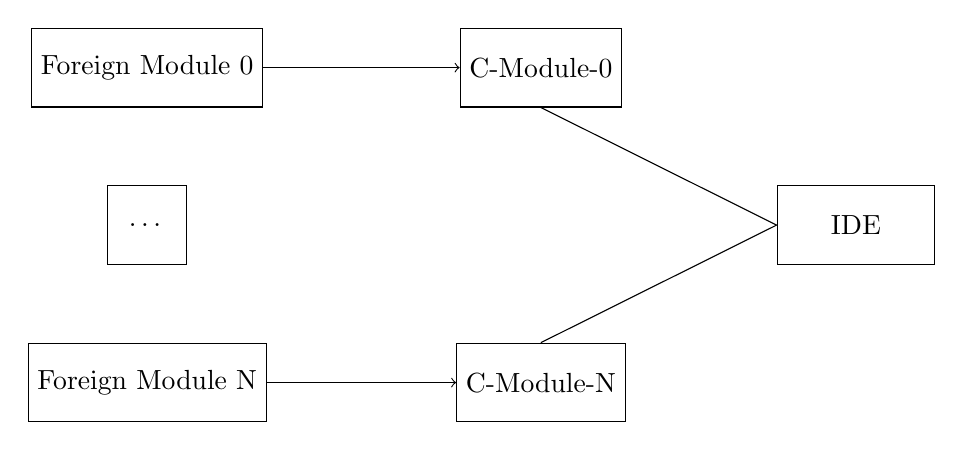
\begin{tikzpicture}
  % Nodes
  \node (p-0) [rectangle, draw, minimum height=1cm, minimum width=2cm] at (-6, 2) {Foreign Module 0};
  \node (dots) [rectangle, draw, minimum height=1cm, minimum width=1cm] at (-6, 0) {\dots};
  \node (p-n) [rectangle, draw, minimum height=1cm, minimum width=2cm] at (-6, -2) {Foreign Module N};
  \node (m-1) [rectangle, draw, minimum height=1cm, minimum width=2cm] at (-1, 2) {C-Module-0};
  \node (m-n) [rectangle, draw, minimum height=1cm, minimum width=2cm] at (-1, -2) {C-Module-N};
  \node (i) [rectangle, draw, minimum height=1cm, minimum width=2cm] at (3, 0) {IDE};
  % Arrow
  \draw (m-1.south) -- (i.west);

  \draw (m-n.north) -- (i.west);

  \draw[->] (p-0) -- (m-1);
  \draw[->] (p-n) -- (m-n);
\end{tikzpicture}

    \caption{Foreign modules being invoked by an individual Translation-module}
    \label{fig:fm2}
  \end{center}
\end{figure}

This module could be a singular one, acting as a translator, translating the
data flowing between the core and foreign-modules as shown in figure
\ref{fig:fm1}, or each foreign-module could have their own translator as shown
in figure \ref{fig:fm2}. For some languages such a setup would be necessary.
A Haskell module, for example, would require some translation module, either a
unique translator for each module, where the Rust module would start the
required Haskell runtime~\cite{ghcRts}, when invoking the Haskell module, and
exit before returning, avoiding \gls*{ub}. The reason Haskell is of interest,
is that the new compiler is written in Haskell~\cite{wiig}, and as such, if one
where to develop \gls*{lsp} capable modules for the \gls*{ide}, a translation
module from Rust to Haskell is necessary.


But this language agnosticism also means that translating from one language to
another should be trivial. This is achieved by the models used in the core. The
\textit{primitive} types, are the same as in JavaScript, the notion of an empty
value, numbers, strings, lists and \textit{objects}, can be
serialized/deserialized to/from any language. So the manipulation on these types
can be extracted and rewritten in another preferred language. Therefore, to be
fully language agnostic, modules should be syntactically translatable between
each other. The same two modules, one implemented in JavaScript, the other in
Rust, should be semantically the same.

\subsection{Existing Third Party Libraries}

Since the core can support different languages, one can use the libraries
written for these languages to make an \gls*{ide}. This could be achieved by
creating a module, acting as a wrapper around the library. For example, by
using JavaScript and since the core application is designed to be an \gls*{ide},
one could use existing JavaScript libraries, like \textit{Monaco}, which is the
text editor used by Visual Studio Code. It comes with an integrated
\gls*{lsp}-client, which would enable the application to easily support existing
popular languages.

However, being zero core, this application could be anything, from an audio
editing program, to a game emulator. Simply using the \textit{JS-DOS} library,
would allow the application to run video games like Doom.

\subsection{Module Development Experience}

A module developer can invoke the module-developer-\gls*{cli}-tool to create
boilerplate modules for JavaScript, TypeScript or Rust. After they have
implemented a module, they can test it out, again by invoking the
\gls*{cli}-tool. When they are satisfied with their implementation, they can add
it to the compile time configuration for the \gls*{ide}, and compile it. They
can now use the module in the \gls*{ide}.

\subsection{Module Tools}

When developing against a module architecture, having tools to help debug issues
is useful. \dots

Some examples of issues we have experienced when developing modules are as
follows:

\begin{itemize}
  \item Incorrect handler registration
  \item Incorrect Event name
  \item Incorrect arguments in response
  \item Incorrect arguments in request
  \item Incorrect State
  \item Concurrent Events
\end{itemize}

Most of these issues relate to the Event system, so being able to mock events
is a useful tool. Luckily, this is quite simple to implement. In
picture \ref{pic:eventMock} we can see this in action.

\begin{figure}[H]
  \centering
  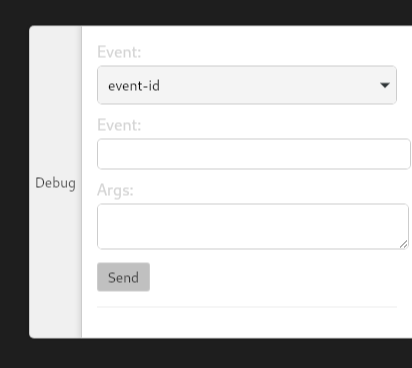
\includegraphics[width=0.5\textwidth]{event-mocking.png}
  \caption{
    Event Mocking module that adds a simple pop-up menu for manually sending
    Events, with specific arguments
  }
  \label{pic:eventMock}
\end{figure}

When mocking in \gls*{rest}-\gls*{api} development, one creates the expected
response, which is usually a \gls*{json}-file. The same is done here, where the
\textit{Args} field in this form expects the argument to be in \gls*{json}. This
is helpful, as other testing libraries, like \textit{Playwright} does the same,
and the \gls*{ide} logs the Event arguments in the same formatting, meaning we
can simply copy-paste the Event argument we want to mock, into the field.

In the picture \ref{pic:debugState}, we can see a module which helps visualize
the current state of the \gls*{ide}, in a tree-graph.

\begin{figure}[H]
  \centering
  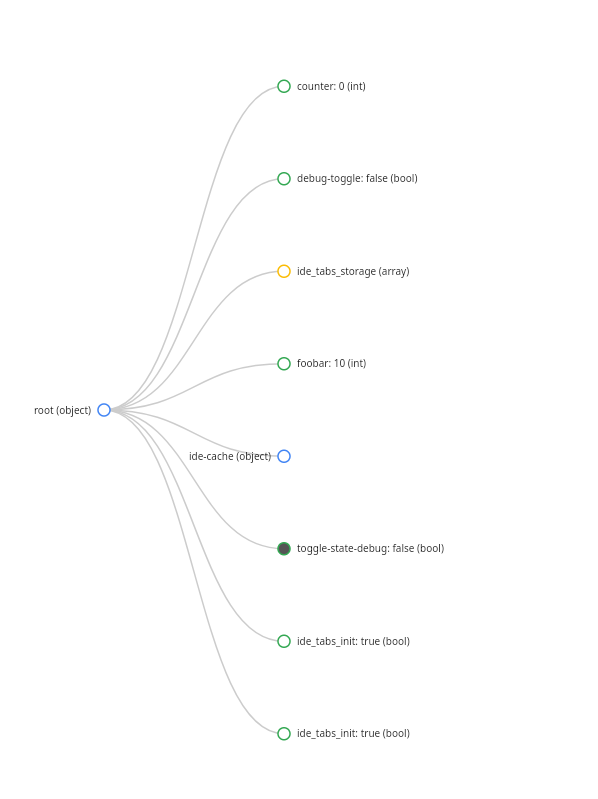
\includegraphics[width=0.75\textwidth]{debug-state.png}
  \caption{
    A module for visualizing the current \gls*{ide}-state
  }
  \label{pic:debugState}
\end{figure}


\subsection{Module Dependency Visualization}

When developing against a modular architecture, it is useful to be able to see
what different module families appear, and what the different dependencies
between the modules are. In picture \ref{pic:modDep} we can see the resulting
graph of the \gls*{ide} modules.

\begin{figure}[H]
  \centering
  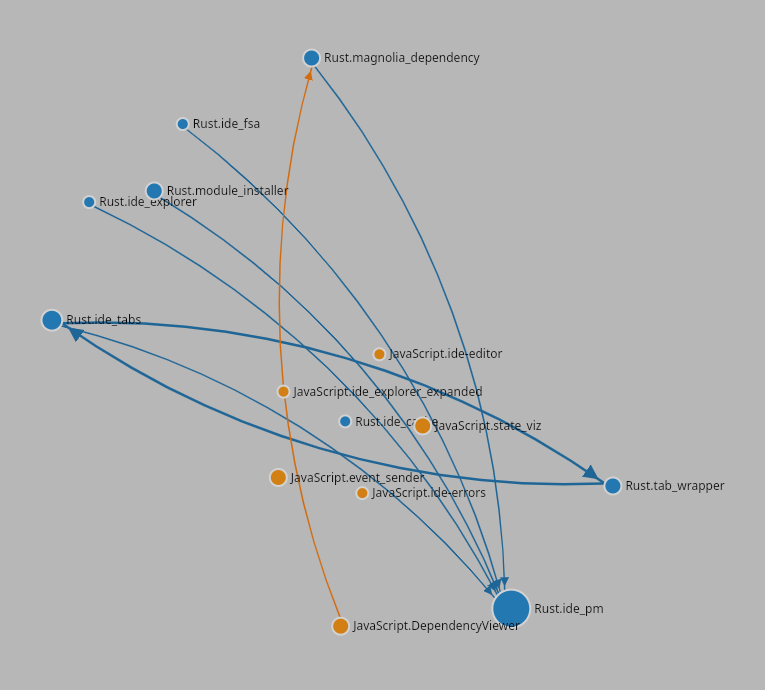
\includegraphics[width=0.75\textwidth]{module-dependencies.png}
  \caption{
    The different modules and their dependencies. Some are coming from an
    unknown source, meaning they subscribe to an Event that has not been
    detected during the analysis
  }
  \label{pic:modDep}
\end{figure}

\section{IDE Users}

As mentioned in chapter \ref{cha:background}, modern \gls*{ide}s come with an
integrated module architecture. Which is used to extend/change the \gls*{ide},
from as simple as to change the theme, to more drastic changes, like changing
all key binds to \textit{vim-motions}. In any case, a user expects certain
functionality to already exist in an \gls*{ide}, like text editing. A maintainer
of a zero core \gls*{ide} could supply modules added at compile time, meaning the
expected functionality is there out of the box, while more thematic modules
could be supplied as runtime modules.

But for more functionality based module, an \gls*{ide} user can make use of the
following modules:

\begin{enumerate}
  \item \textit{ide\_explorer}: Responsible for the file explorer
  \item \textit{ide\_framework}: Responsible for general layout
  \item \textit{ide\_pm}: Responsible for the menu bar
  \item \textit{ide\_tabs}: Responsible for the tabbing system
  \item \textit{ide\_errors}: Responsible in displaying module errors
\end{enumerate}

In the figure \ref{fig:ideLayout}, we have laid out the naming convention we
use when referring to different \textit{places} in the \gls*{ide}.

\begin{figure}[H]
  \centering
  \begin{tikzpicture}
  \node (window) [rectangle, draw, minimum height=7cm, minimum width=10cm] at (0, 0) {};
  \node (menu) [rectangle, draw, minimum height=0.5cm, minimum width=10cm] at (0, 3.25) {Menu};
  \node (tabs) [rectangle, draw, minimum height=0.25cm, minimum width=8cm] at (1, 2.75) {Tabs};
  \node (tab) [rectangle, draw, minimum height=0.25cm, minimum width=1cm] at (-2.5, 2.75) {Tab};
  \node (sidebar) [rectangle, draw, minimum height=6.5cm, minimum width=2cm] at (-4, -0.25) {Sidebar};
  \node (content) [rectangle, draw, minimum height=6.5cm, minimum width=8cm] at (1, -0.25) {Content};
\end{tikzpicture}
  \caption{\gls*{ide} layout}
  \label{fig:ideLayout}
\end{figure}

\paragraph{ide\_explorer} In picture \ref{pic:ideEx} we can see the
\textit{ide\_explorer} in action, showing the Magnolia library visualized as a
tree-like structure with collapsible folders. These folders are rendered in the
\textit{sidebar}, on the left. When we click on the \textit{File}, a dropdown
appears, where we can click on a button, \textit{Open Folder}, which sends an
Event to \gls*{ide}\_fsa, the module in charge of handling file system
operations, where we get in \textit{response}, all the folders and files in the
path we selected. Which we transform into \gls*{html}, and along with some
\gls*{css}, we get the collapsible folders.

\paragraph{ide\_framework} \dots

\paragraph{ide\_pm}, being responsible for the menu bar at the top of the
\gls*{ide}, has an \textit{easy} job, as it just simplifies the creation of
interactive \gls*{ui} elements for other modules. With the dependency graph
visualization module, we can create a module which sends the initial Event that
triggers the graph visualization, and have the button be under the \textit{View}
dropdown content.

\begin{figure}
  \centering
  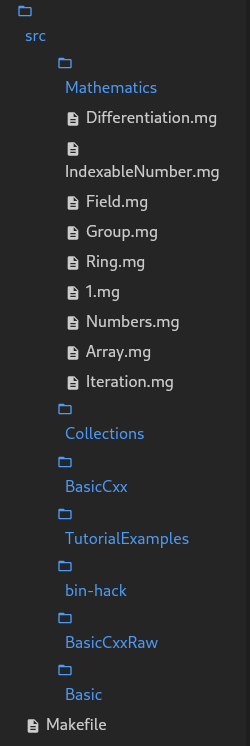
\includegraphics[height=0.5\textwidth]{ide-explorer.png}
  \caption{
    \gls*{ide}-explorer module, showing the Magnolia library.
  }
  \label{pic:ideEx}
\end{figure}

\subsection{Editor Module Family}

The editor module family is coupled with the \gls*{ide} framework, as using the
ide\_explorer module, we can open and edit files. By adding a \textit{click}
attribute to the files in the tree, we send an Event to \gls*{ide}\_fsa, which
reads the file we clicked on. We know what file we clicked on, because each
\textit{click} attribute has sends an Event with their corresponding path. When
we get the texts contents of the file in response, we create an textarea with
the contents of the file added to it. In picture \ref{pic:editorModule} we can
see this in action, as the editor is created in the \textit{content} place, in
the center of the \gls*{ide}, along with a \textit{tab}, with the name of the
file being edited as the title of the tab.

\begin{figure}
  \centering
  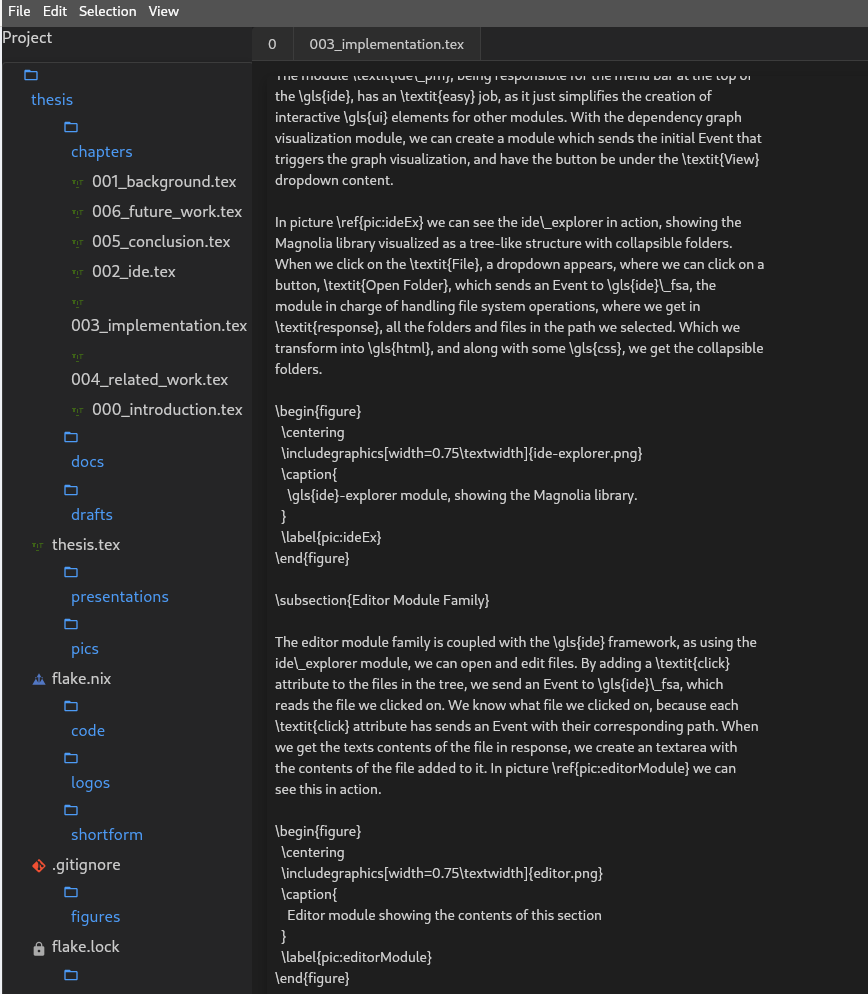
\includegraphics[width=0.5\textwidth]{editor.png}
  \caption{
    Editor module showing the contents of this section
  }
  \label{pic:editorModule}
\end{figure}


\subsection{Magnolia Dependency Graph Visualizer}

In Magnolia, as in many other languages, one cannot have a cyclic dependency.
This means that the dependency graph of a Magnolia project should be a
\gls*{dag}. And since Magnolia has such a focus on reuse, the dependency graphs
in a Magnolia project could be quite large. Which means the cycles could be
quite long, which would make resolving the cyclic dependency issue complicated.
One way to help a developer, would be to give them a tool to visualize the
dependency graph, so that they could see what modules are connected. Using the
Magnolia library as the input, we can create a visualization of the dependencies
in Magnolia. Using two modules, one for \textit{parsing} the Magnolia library,
finding all packages, and their dependencies, and another for visualizing
this.

The module responsible for rendering the graph, uses
\textit{D3}\footnote{\url{https://d3js.org/}}, a visualization library for
JavaScript. In the picture \ref{pic:magLib}, we can see the finished rendering
of the dependency graph of the Magnolia basic library. As mentioned earlier,
Magnolia has a lot of re-use, and therefore dependencies. That makes this
visualization quite \textit{noisy}, as there are a lot of crossing between the
dependencies.

\begin{figure}[H]
  \centering
  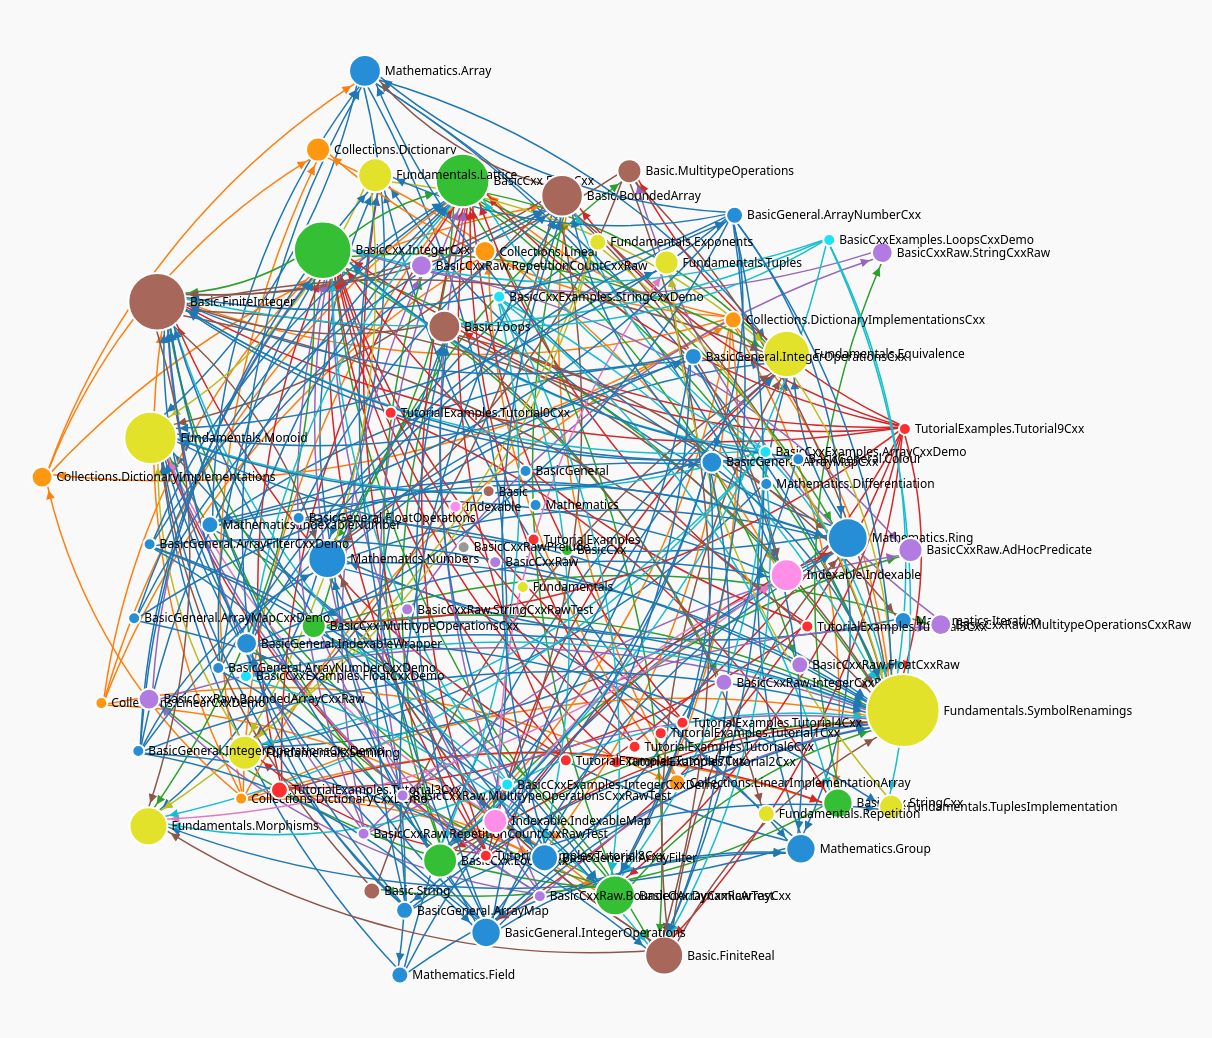
\includegraphics[width=0.75\textwidth]{magnolia-dependencies.png}
  \caption{
    Magnolia basic library dependencies visualized in the \gls*{ide} using
    modules. Each colour represents a package, which contains several modules.
    The size of the nodes vary depending on the amount of dependents,
    (in degree), a module has.
  }
  \label{pic:magLib}
\end{figure}

Luckily, with \textit{D3}, we can mitigate some of the noise. In the picture
\ref{pic:depCont}, we can see the control-panel that our graph module has
created. With the control panel, we can zoom in and out on the graph,~\footnote{This can also be done with the mouse}
reset our view. This, along with the node size scale, scaling how big
a node is depending on how many dependents it has, ensures this visualization
tool can be used for other programming libraries, not just Magnolia.\footnote{Given a proper parser module}

\begin{figure}[H]
  \centering
  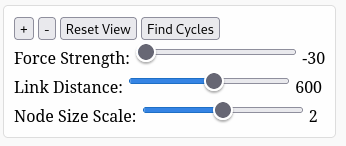
\includegraphics[width=0.45\textwidth]{dependency-viewer-controls.png}
  \caption{
    Control panel, with buttons and sliders for controlling the graph view
  }
  \label{pic:depCont}
\end{figure}

Furthermore, we can highlight the packages we care about, using the filter
panel the module created. In picture \ref{pic:depFil}, all the different
Magnolia packages have been detected, and their corresponding colour has been
added. We can then enable, or disable them.

\begin{figure}[H]
  \centering
  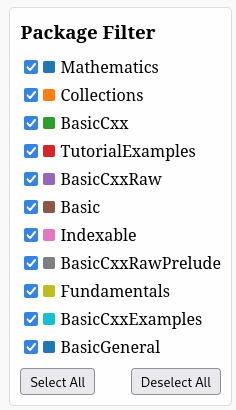
\includegraphics[height=0.5\textwidth]{dependency-viewer-filter.png}
  \caption{List of packages in the graph, that can be toggled}
  \label{pic:depFil}
\end{figure}

In the picture \ref{pic:depDis}, we can see the graph after we have disabled all
other packages, except the \textit{Fundamentals} package.

\begin{figure}[H]
  \centering
  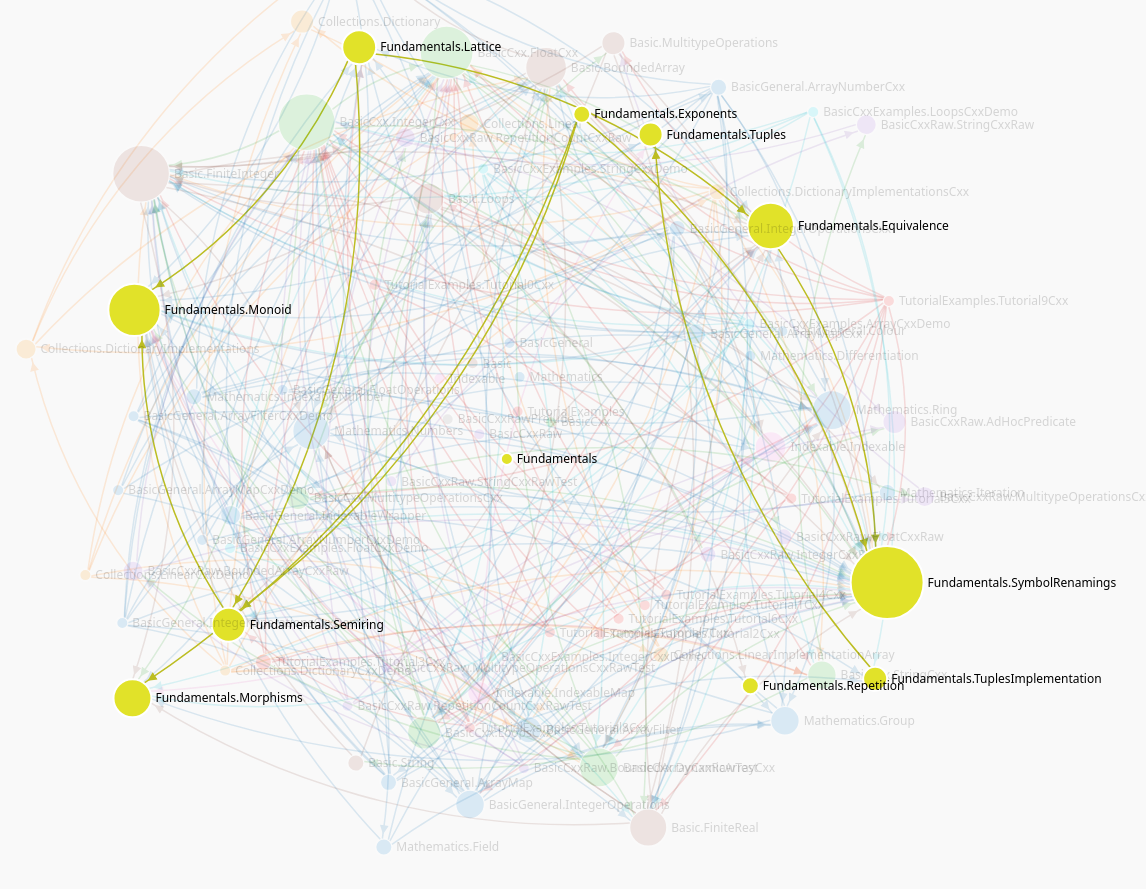
\includegraphics[width=0.75\textwidth]{magnolia-dependencies-filtered.png}
  \caption{
    Magnolia basic library, with just the \textit{Fundamentals} package
    highlighted.
  }
  \label{pic:depDis}
\end{figure}


\subsection{Developer}

Most users just want an \gls*{ide}, and do not spend, nor want to spend, much
time configuring their \gls*{ide}. This can be achieved by adding the necessary
modules to qualify as an \gls*{ide} at compile time. If one is a lecturer,
teaching something that is used by a \textit{niche} programming language, the
lecturer can add the needed modules to a configuration file,
\textit{Modules.toml}, and then compile it to an \gls*{ide}. Before the \gls*{ide}
is compiled, it finds the mentioned modules in the configuration file, and
directly integrates them into the core, ensuring that the resulting binary is a
fully fledged \gls*{ide}. And then this \gls*{ide} can be distributed to the
students, who can still extend the \gls*{ide} with runtime modules at their own
digression.

\subsection{Module Installer}

Module markets are an important part of the \gls*{ide} user experience. Being
able to install a module with the click of a button essential. Not having a
dedicated module market like \gls*{vscode}, has not been detrimental for
\gls*{vim}, as with a \textit{plugin manager}, a user can install a module by
simply supplying a URL to a GitHub repository. Similarly, we allow users to
either install modules from disk, or by supplying a URL to a GitHub repository.
In the picture \ref{pic:moduleInstaller}, we can see such a form. A user can
either install a module from disk, in which case, we simply copy the module
binary at the given path to the runtime module folder, or if a URL has been
supplied, we get the latest released binary from that GitHub repository, and
copy this binary instead.

\begin{figure}
  \centering
  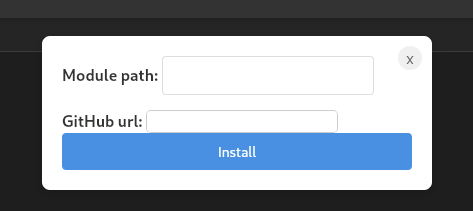
\includegraphics[width=0.50\textwidth]{module-installer.png}
  \caption{
    A module installation form, where a user can supply a path to a module on
    disk, or a URL to a GitHub repository containing the module binary.
  }
  \label{pic:moduleInstaller}
\end{figure}


\section{Maintainer}

To make the maintainer of the core application most comfortable, good
documentation is needed. The same documentation a module developer wants, so
it's important for them and the maintainer that the documentation is up-to-date.
But how good is documentation if it is not updated when the code being
documented is changed? This is where Rust's doc-test system comes into play. Any
function annotated with a doc string, can contain code examples. If these code
examples are written as Rust code, and use assert statements, then this code is
run, during testing, as if it was an actual test. Meaning the saying
\textit{code is documentation}, is \textit{documentation is code} in Rust.

\subsection{Testing}

Ensuring the core library used by module developers is correct, is an essential
part of a maintainers job. The easiest way for a maintainer to achieve this, is
to test in production; letting module developers report issues. This is not a
good experience for module developers. But the second-easiest way is to create
unit tests that ensure edge cases are handled correctly. We have designed test
data for serializing and deserializing data between the different languages
supported by the \gls{ide}, ensuring that any library developed can be
verified to work correctly. The test data is modular, meaning we can easily
create new edge cases. In the picture \ref{pic:libTest}, we can see that there
are $135$ different test cases.

\begin{figure}
  \centering
  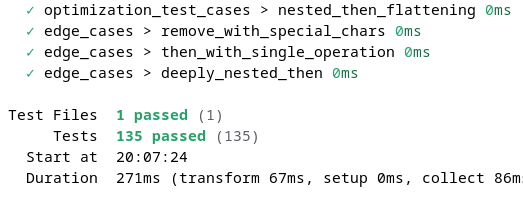
\includegraphics[width=0.50\textwidth]{libtest.png}
  \caption{Picture showing the output of running the test data}
  \label{pic:libTest}
\end{figure}
